\documentclass[14pt]{extbook}
\usepackage{multicol, enumerate, enumitem, hyperref, color, soul, setspace, parskip, fancyhdr} %General Packages
\usepackage{amssymb, amsthm, amsmath, latexsym, units, mathtools} %Math Packages
\everymath{\displaystyle} %All math in Display Style
% Packages with additional options
\usepackage[headsep=0.5cm,headheight=12pt, left=1 in,right= 1 in,top= 1 in,bottom= 1 in]{geometry}
\usepackage[usenames,dvipsnames]{xcolor}
\usepackage{dashrule}  % Package to use the command below to create lines between items
\newcommand{\litem}[1]{\item#1\hspace*{-1cm}\rule{\textwidth}{0.4pt}}
\pagestyle{fancy}
\lhead{Progress Quiz 7}
\chead{}
\rhead{Version B}
\lfoot{4173-5738}
\cfoot{}
\rfoot{Spring 2021}
\begin{document}

\begin{enumerate}
\litem{
Solve the radical equation below. Then, choose the interval(s) that the solution(s) belongs to.\[ \sqrt{30 x^2 + 81} - \sqrt{-99 x} = 0 \]\begin{enumerate}[label=\Alph*.]
\item \( x_1 \in [-2.32, -1.77] \text{ and } x_2 \in [-4.5,-0.5] \)
\item \( x \in [-2.32,-1.77] \)
\item \( x_1 \in [1.41, 1.67] \text{ and } x_2 \in [-0.2,3.8] \)
\item \( \text{All solutions lead to invalid or complex values in the equation.} \)
\item \( x \in [-1.78,-1.24] \)

\end{enumerate} }
\litem{
Choose the equation of the function graphed below.
\begin{center}
    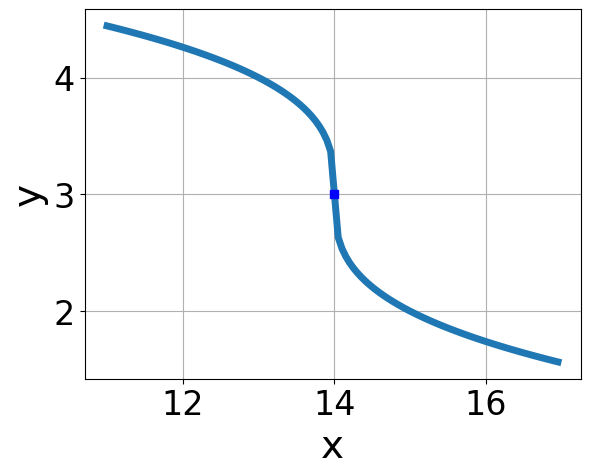
\includegraphics[width=0.5\textwidth]{../Figures/radicalGraphToEquationB.png}
\end{center}
\begin{enumerate}[label=\Alph*.]
\item \( f(x) = \sqrt[3]{x - 14} + 3 \)
\item \( f(x) = \sqrt[3]{x + 14} + 3 \)
\item \( f(x) = - \sqrt[3]{x - 14} + 3 \)
\item \( f(x) = - \sqrt[3]{x + 14} + 3 \)
\item \( \text{None of the above} \)

\end{enumerate} }
\litem{
Solve the radical equation below. Then, choose the interval(s) that the solution(s) belongs to.\[ \sqrt{-15 x^2 + 56} - \sqrt{19 x} = 0 \]\begin{enumerate}[label=\Alph*.]
\item \( x_1 \in [1.4, 3.4] \text{ and } x_2 \in [1.7,3] \)
\item \( x_1 \in [-3.67, 0.33] \text{ and } x_2 \in [0.1,2.4] \)
\item \( \text{All solutions lead to invalid or complex values in the equation.} \)
\item \( x \in [1.4,3.4] \)
\item \( x \in [-3.67,0.33] \)

\end{enumerate} }
\litem{
Choose the graph of the equation below.\[ f(x) = \sqrt{x + 8} + 4 \]\begin{enumerate}[label=\Alph*.]
\begin{multicols}{2}\item 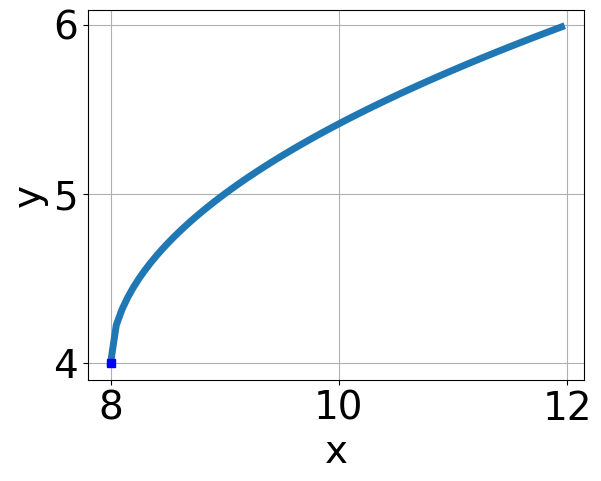
\includegraphics[width = 0.3\textwidth]{../Figures/radicalEquationToGraphAB.png}\item 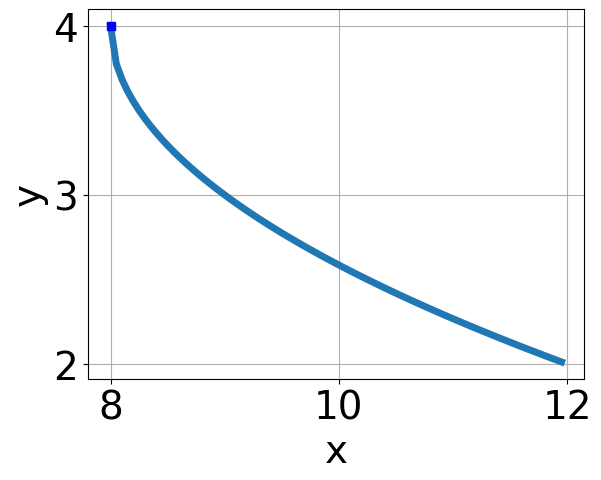
\includegraphics[width = 0.3\textwidth]{../Figures/radicalEquationToGraphBB.png}\item 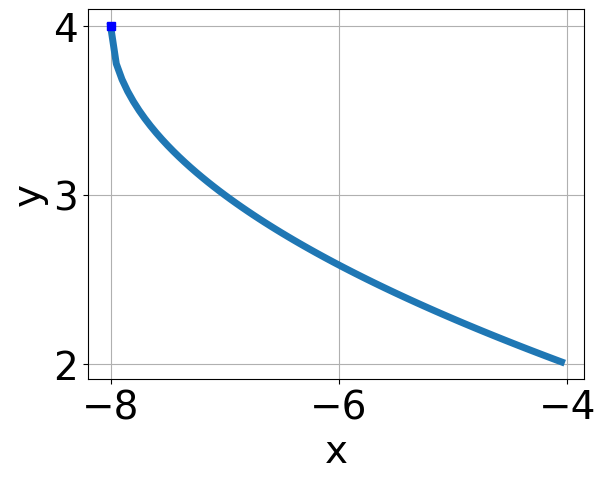
\includegraphics[width = 0.3\textwidth]{../Figures/radicalEquationToGraphCB.png}\item 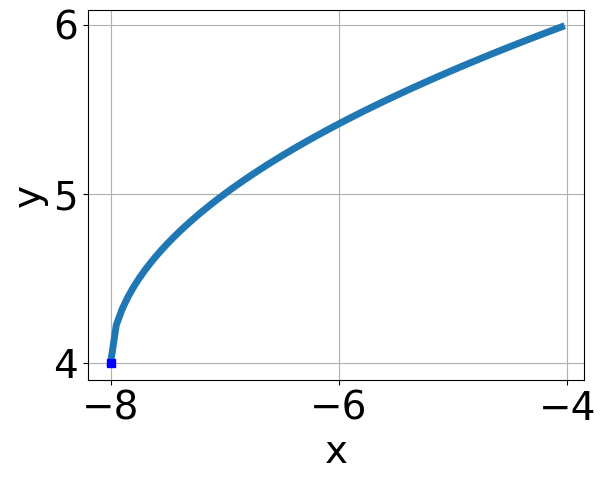
\includegraphics[width = 0.3\textwidth]{../Figures/radicalEquationToGraphDB.png}\end{multicols}\item None of the above.
\end{enumerate} }
\litem{
Solve the radical equation below. Then, choose the interval(s) that the solution(s) belongs to.\[ \sqrt{6 x - 9} - \sqrt{7 x + 8} = 0 \]\begin{enumerate}[label=\Alph*.]
\item \( x_1 \in [-17.6, -16.75] \text{ and } x_2 \in [-0.5,5.5] \)
\item \( x \in [-17.6,-16.75] \)
\item \( \text{All solutions lead to invalid or complex values in the equation.} \)
\item \( x_1 \in [-1.75, -1.08] \text{ and } x_2 \in [-0.5,5.5] \)
\item \( x \in [-1.12,-0.97] \)

\end{enumerate} }
\litem{
Choose the graph of the equation below.\[ f(x) = \sqrt[3]{x - 8} - 3 \]\begin{enumerate}[label=\Alph*.]
\begin{multicols}{2}\item 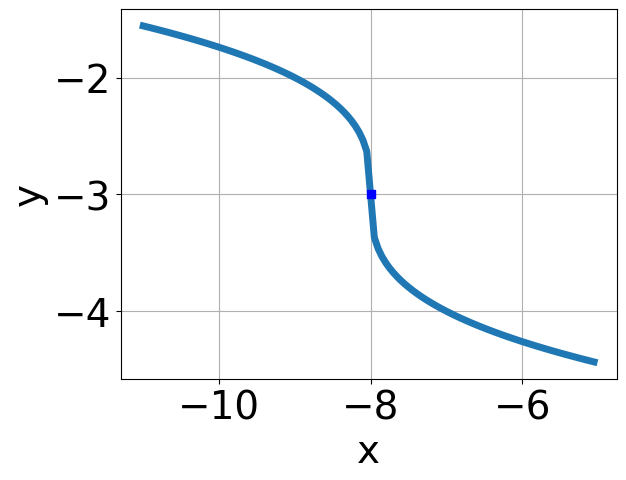
\includegraphics[width = 0.3\textwidth]{../Figures/radicalEquationToGraphCopyAB.png}\item 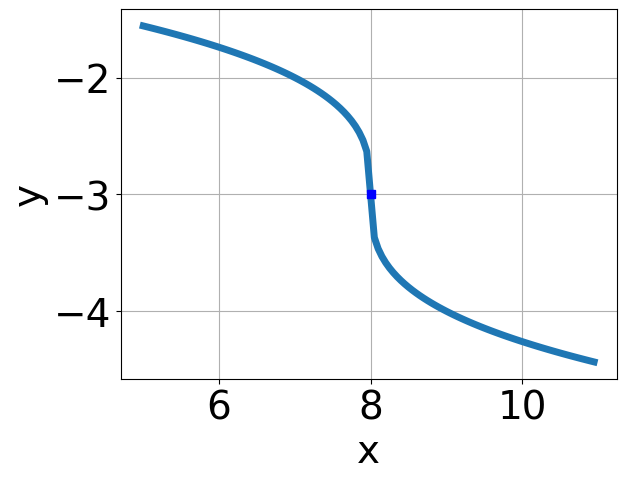
\includegraphics[width = 0.3\textwidth]{../Figures/radicalEquationToGraphCopyBB.png}\item 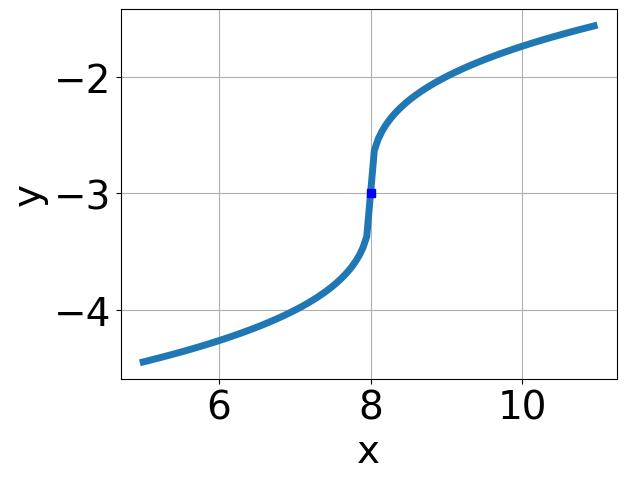
\includegraphics[width = 0.3\textwidth]{../Figures/radicalEquationToGraphCopyCB.png}\item 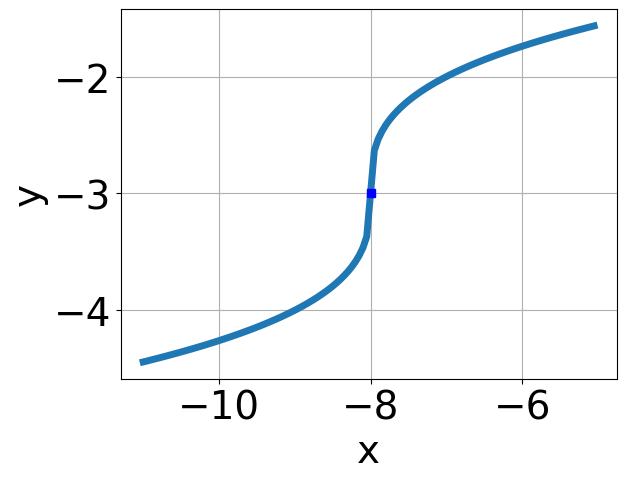
\includegraphics[width = 0.3\textwidth]{../Figures/radicalEquationToGraphCopyDB.png}\end{multicols}\item None of the above.
\end{enumerate} }
\litem{
What is the domain of the function below?\[ f(x) = \sqrt[4]{-6 x + 8} \]\begin{enumerate}[label=\Alph*.]
\item \( (-\infty, a], \text{where } a \in [-0.15, 1] \)
\item \( (-\infty, a], \text{ where } a \in [1.16, 1.39] \)
\item \( [a, \infty), \text{where } a \in [1.1, 1.9] \)
\item \( [a, \infty), \text{where } a \in [-1.1, 1] \)
\item \( (-\infty, \infty) \)

\end{enumerate} }
\litem{
What is the domain of the function below?\[ f(x) = \sqrt[8]{4 x - 5} \]\begin{enumerate}[label=\Alph*.]
\item \( [a, \infty), \text{where } a \in [0.09, 0.96] \)
\item \( (-\infty, a], \text{where } a \in [1.19, 1.38] \)
\item \( (-\infty, a], \text{where } a \in [0.71, 1.24] \)
\item \( [a, \infty), \text{ where } a \in [1.19, 1.28] \)
\item \( (-\infty, \infty) \)

\end{enumerate} }
\litem{
Solve the radical equation below. Then, choose the interval(s) that the solution(s) belongs to.\[ \sqrt{4 x - 7} - \sqrt{7 x - 6} = 0 \]\begin{enumerate}[label=\Alph*.]
\item \( x \in [-1.4,0.3] \)
\item \( x_1 \in [-1.4, 0.3] \text{ and } x_2 \in [0.75,6.75] \)
\item \( x \in [-4.8,-3.6] \)
\item \( x_1 \in [0.5, 1.6] \text{ and } x_2 \in [0.75,6.75] \)
\item \( \text{All solutions lead to invalid or complex values in the equation.} \)

\end{enumerate} }
\litem{
Choose the equation of the function graphed below.
\begin{center}
    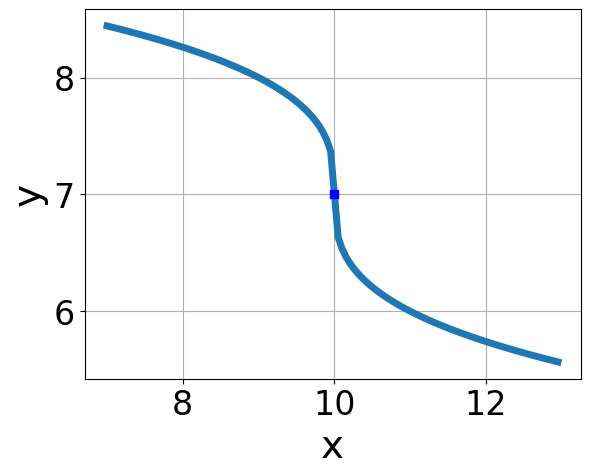
\includegraphics[width=0.5\textwidth]{../Figures/radicalGraphToEquationCopyB.png}
\end{center}
\begin{enumerate}[label=\Alph*.]
\item \( f(x) = \sqrt[3]{x + 10} + 7 \)
\item \( f(x) = - \sqrt[3]{x + 10} + 7 \)
\item \( f(x) = \sqrt[3]{x - 10} + 7 \)
\item \( f(x) = - \sqrt[3]{x - 10} + 7 \)
\item \( \text{None of the above} \)

\end{enumerate} }
\end{enumerate}

\end{document}